\renewcommand{\CODELOC}{c/ch4/}

\chapter{Nonlinear elliptic PDEs on structured grids}
\label{chap:nonlinear}

\section{Newton's method}

FIXME suppose $\bF : \RR^N \to \RR^N$ is differentiable.  note $\bF(\bx) = [F_0(\bx), \dots, F_{N-1}(\bx)]$, which we regard as a column vector.  to solve
\begin{equation}
   \bF(\bx) = 0.   \label{eq:nl:equation}
\end{equation}

given $\bx_k$ and $\Delta\bx$, define $\bx_{k+1} = \bx_k + \Delta\bx$.  note that if $\bF$ is a smooth function then
\begin{equation}
    \bF(\bx_{k+1}) = \bF(\bx_k) + J_\bF(\bx_k) \Delta\bx + O(\|\Delta\bx\|^2)  \label{eq:nl:expandF}
\end{equation}
where
\begin{equation}
J_\bF(\bx) = \begin{bmatrix}
    \frac{\partial F_0}{\partial x_0} & \dots & \frac{\partial F_0}{\partial x_{N-1}} \\
    \vdots & \ddots & \vdots \\
    \frac{\partial F_{N-1}}{\partial x_0} & \dots & \frac{\partial F_{N-1}}{\partial x_{N-1}}  \end{bmatrix}  \label{eq:nl:jacdefn}
\end{equation}
is the Jacobian matrix of $\bF$ at $\bx$.

Newton's method is an iteration which solves nonlinear equation \eqref{eq:nl:equation} by linearization from truncating \eqref{eq:nl:expandF}.  each step computes $\Delta x$ so that $\bF(\bx_{k+1})=0$ in \eqref{eq:nl:expandF}, after dropping the $O(\|\Delta\bx\|^2)$ term, i.e.~we solve
\begin{equation}
    0 = \bF(\bx_k) + J_\bF(\bx_k) \Delta\bx
\end{equation}
for $\Delta x$.  thus at each iteration $k$ we solve a linear system and then do a vector update:
\begin{align}
    J_\bF(\bx_k) \Delta\bx &= - \bF(\bx_k)  \label{eq:nl:Newton}  \\
    \bx_{k+1} &= \bx_k + \Delta\bx  \notag
\end{align}
This is fairly-simple in theory.

In practice is not \emph{that} much more complicated, despite the reputation of Newton iteration as fragile or scary.  Let's see an example:

\medskip\noindent\hrulefill
\begin{example}  Nonlinear systems can be thought of as describing the intersections of curves, surfaces, or hypersurfaces, depending on dimension.  For example, this pair of nonlinear equations
    $$y = \frac{1}{2} e^x, \qquad x^2+y^2 = 1$$
are an exponential curve and a circle around the origin.  They are easy to visualize, and also shown in Figure FIXME.  The curves clearly have two points of intersection, one each in the first and second quadrants.  Finding those points of intersection means solving the system of simultaneous nonlinear equations.

To put the system in standard form \eqref{eq:nl:equation} we write
\begin{equation}
\bF(\bx) = \begin{bmatrix}
           e^{x_0} - 2 x_1 \\
           x_0^2 + x_1^2 - 1
           \end{bmatrix}
\end{equation}
for $\bx\in \RR^2$.  Thus
\begin{equation}
J_\bF(\bx) = \begin{bmatrix}
    e^{x_0} & -2 \\
    2 x_0   & 2 x_1 \end{bmatrix}
\end{equation}
If we start the Newton iteration with $\bx_0 = [1,1]$ then the sequence of iterates from \eqref{eq:nl:Newton} is
    $$\twovect{\bx}{0}{1}{1}, \twovect{\bx}{1}{FIXME}{FIXME}, \dots$$
as shown in Figure FIXME
\end{example}
\noindent\hrulefill

\medskip
There are only two main ideas, beyond the construction of the Newton iteration \eqref{eq:nl:Newton} itself, which turn Newton iteration into an effective, indeed profoundly-effective, tool:
\renewcommand{\labelenumi}{\roman{enumi})}
\begin{enumerate}
\item FIXME linesearch or trust region needed \citep{Kelley2003}
\item FIXME full range of linear tools (e.g.~Chapter \ref{chap:linearsystem}) should be applied to the linear system \eqref{eq:nl:Newton}
\end{enumerate}

What make's Newton so good?  FIXME: quadratic convergence


\section{\pSNES and call-backs}

FIXME  we solve the above example in code \texttt{expcircle.c} as shown in Figure \ref{code:expcircle}.  this is the entire code, but note that the Jacobian $J_\bF(\bx)$ is not implemented in code.  run it
\begin{cline}
$ cd c/ch4/
$ make expcircle
$ ./expcircle -snes_fd
\end{cline}
%$
Better is to add option \texttt{-snes\_monitor}.  Also \texttt{-snes\_mf} works.

FIXME the code works through \emph{call-back}.  Specifically FIXME

\vfill
\cinput{expcircle.c}{\CODELOC}{FIXME}{//START}{//END}{code:expcircle}


\section{Jacobians, exact and approximate}

FIXME

\vfill
\cinputpart{expcircleJAC.c}{\CODELOC}{FIXME}{I}{//STARTJAC}{//ENDJAC}{code:expcircleJACI}

\cinputpart{expcircleJAC.c}{\CODELOC}{FIXME}{II}{//STARTADDJAC}{//ENDADDJAC}{code:expcircleJACII}


\section{Example: 1D reaction-diffusion equation}

FIXME

\vfill
\cinputpart{reaction.c}{\CODELOC}{FIXME}{I}{//SETUP}{//ENDSETUP}{code:reactionI}

\cinputpart{reaction.c}{\CODELOC}{FIXME}{II}{//FUNCTION}{//ENDFUNCTION}{code:reactionII}

\cinputpart{reaction.c}{\CODELOC}{FIXME}{III}{//JACOBIAN}{//ENDJACOBIAN}{code:reactionIII}

\cinputpart{reaction.c}{\CODELOC}{FIXME}{IV}{//MAIN}{//ENDMAIN}{code:reactionIV}

\section{Optimization and nonlinear PDEs: $p$-Laplacian equation}

FIXME for $p>1$,
    $$I[u] = \int_\Omega \frac{1}{p} |\grad u|^p - fu$$
the variational equation is the weak form of a PDE:
\begin{align*}
I[u+\eps v] - I[u] &= \int_\Omega \frac{1}{p} |\grad u + \eps \grad v|^p + \frac{1}{p} |\grad u|^p - \eps f v \\
   &= \eps \left(\int_\Omega |\grad u|^{p-2} \grad u \cdot \grad v - f v\right) + O(\eps^2)
\end{align*}
so we want
    $$0 = \int_\Omega |\grad u|^{p-2} \grad u \cdot \grad v - f v$$
for all $v \in W^{1,p}_0(\Omega)$.  this can become a strong form by another integration by parts,
    $$0 = - \Div\left(|\grad u|^{p-2} \grad u\right) - f$$
which is \eqref{poissonsquare} if $p=2$

FIXME introduce $Q^1$ FEM on structured grid

\begin{marginfigure}
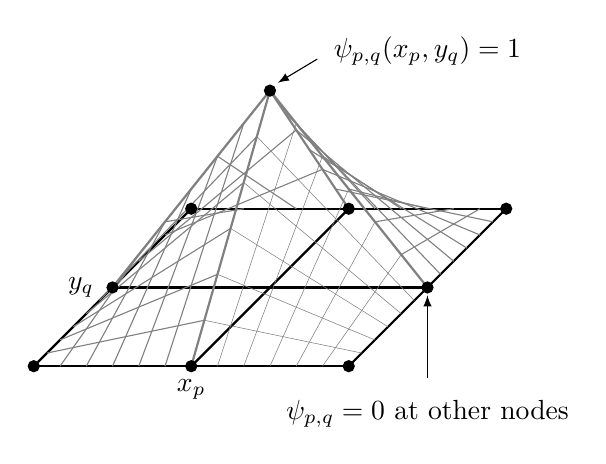
\begin{tikzpicture}[scale=0.5]

  % strong grid around elements
  \draw[thick] (0,0) -- (8,0);
  \draw[thick] (2,2) -- (10,2);
  \draw[thick] (4,4) -- (12,4);
  \draw[thick] (0,0) -- (4,4);
  \draw[thick] (4,0) -- (8,4);
  \draw[thick] (8,0) -- (12,4);

  \def\ytop{7};

  % tent lines
  \draw[gray,thick] (6,\ytop) -- (4,0);
  \draw[gray,thick] (6,\ytop) -- (2,2);
  \draw[gray,thick] (6,\ytop) -- (10,2);
  \draw[gray,thick] (6,\ytop) -- (8,4);

  \def\dx{(10.0-6.0)/6};
  \def\dy{(2.0-\ytop)/6};
  \foreach \jj in {1,...,5}
  {
       \draw[gray,very thin] ({6+\jj*\dx},{\ytop+\jj*\dy}) -- ({4+(4/6)*\jj},0.0);
  }

  \def\dx{(4.0-6.0)/6};
  \def\dy{(0.0-\ytop)/6};
  \foreach \jj in {1,...,5}
  {
       \draw[gray,very thin] ({6+\jj*\dx},{\ytop+\jj*\dy}) -- ({10-(2/6)*\jj},{2-(2/6)*\jj});
  }

  \def\dx{(2.0-6.0)/6};
  \def\dy{(2.0-\ytop)/6};
  \foreach \jj in {1,...,5}
  {
       \draw[gray,thin] ({6+\jj*\dx},{\ytop+\jj*\dy}) -- ({4-(4/6)*\jj},0.0);
  }

  \def\dx{(4.0-6.0)/6};
  \def\dy{(0.0-\ytop)/6};
  \foreach \jj in {1,...,5}
  {
       \draw[gray,thin] ({6+\jj*\dx},{\ytop+\jj*\dy}) -- ({2-(2/6)*\jj},{2-(2/6)*\jj});
  }

  \def\dx{(10.0-6.0)/6};
  \def\dy{(2.0-\ytop)/6};
  \foreach \jj in {1,...,5}
  {
       \draw[gray,thin] ({6+\jj*\dx},{\ytop+\jj*\dy}) -- ({8+(4/6)*\jj},4.0);
  }

  \def\dx{(8.0-6.0)/6};
  \def\dy{(4.0-\ytop)/6};
  \foreach \jj in {1,...,5}
  {
       \draw[gray,thin] ({6+\jj*\dx},{\ytop+\jj*\dy}) -- ({10+(2/6)*\jj},{2+(2/6)*\jj});
  }

  \def\dx{(2.0-6.0)/3};
  \def\dy{(2.0-\ytop)/3};
  \foreach \jj in {1,...,2}  % reduce clutter
  {
       \draw[gray,thin] ({6+\jj*\dx},{\ytop+\jj*\dy}) -- ({8-(4/3)*\jj},4.0);
  }

  \def\dx{(8.0-6.0)/3};
  \def\dy{(4.0-\ytop)/3};
  \foreach \jj in {1,...,2}
  {
       \draw[gray,thin] ({6+\jj*\dx},{\ytop+\jj*\dy}) -- ({2+(2/3)*\jj},{2+(2/3)*\jj});
  }

  % nodes in base plane
  \filldraw (0,0) circle (4pt);
  \filldraw (4,0) circle (4pt);
  \filldraw (8,0) circle (4pt);
  \filldraw (2,2) circle (4pt);
  %\filldraw (6,2) circle (4pt);   % (x_j,y_k) is at (6,2)
  \filldraw (10,2) circle (4pt);
  \filldraw (4,4) circle (4pt);
  \filldraw (8,4) circle (4pt);
  \filldraw (12,4) circle (4pt);

  % node at tent top
  \filldraw (6,\ytop) circle (4pt);

  % annotate
  \draw (10,\ytop+1.0) node {$\psi_{p,q}(x_p,y_q)=1$};
  \draw[-latex] (7.2,\ytop+0.8) -- (6.2,\ytop+0.2);
  \draw (10,-1.2) node {$\psi_{p,q}=0$ at other nodes};
  \draw[-latex] (10,-0.3) -- (10,1.8);

  % label center point
  \draw (4,-0.6) node {$x_p$};
  \draw (1.2,2) node {$y_q$};

\end{tikzpicture}

\caption{FIXME}
\label{fig:q1hat}
\end{marginfigure}

FIXME code uses \texttt{SNESSetObjective()} only, though also \texttt{SNESSetFunction()}; no hand-made Jacobian at all

FIXME try NCG
